\section{Introduction}

%% 
%% Leave first page empty
\thispagestyle{empty}

The need of a new way to communicate between two points of the planet has been arising as a problem to be solved by our new media distributors. Old systems such as Skype or traditional video calls are not able to cope the needs of the new generations of developers and users that everyday require a more integrated way of communication. 

Besides this, the amount of data being transferred during the last years and the prevision for the future allocates a new scenario where non-centralized systems such as P2P are required as data bandwidth grows and systems need to become more scalable. Nowadays networks are still manly content-centric, meaning that data is provided from a source to a client in a triangle scheme, clients upload data to central servers and this data is transferred to the endpoint. This architecture has been provided since long time as reliable and scalable, but with the appearance of powerful applications and media transfer it has been proven to become a real problem.

Those circumstances lead to a whole new world of real-time browser based applications which require also a totally new framework to be developed into. Starting from the online videoconferencing to real-time data applications, for this purpose few attempts where made in the past being highly reliable on specific hardware and custom-built no-compatible system. Taking these decisions made those proposals not be accessible by the massive amount of normal users that could not afford to adapt the requirements. 

All the previous concepts are now possible thanks to the increase of performance related to the hardware components available in every 
average computer nowadays, this increase has helped to build more complex browsers that are able to perform many tasks not just related 
to web browsing. Having a browser handling OpenGL style of applications is now possible thank to the increase of performance. Besides this multimedia abilities have also been able to reproduce on those browsers and handling webcam media as html is now a reality. Even dough there are still some issues to be considered before being able to freely communicate between two browsers: there is no common standardized protocol that allows developers to do this. WebRTC goal is to approach this problem to build a simple and standard solution for peer-to-peer browser communication \cite{alvestrandOverview2012}.

Internet bandwidth has helped to take the decision to start integrating peer-to-peer solutions in browsed based applications, this is due the year-by-year increase of user bandwidth connectivity during the last 10 years. As before the latency was too high being unable to maintain real-time applications working resiliently. But recently the amount of users being able to transfer at high speed has been rapidly increasing as you can see in the following figure, about 39\% of users are now able to download at speeds greater than 4Mbps being this a very good average speed for media content \cite{akamaiq2}.

\begin{figure}[h]
  \centering
    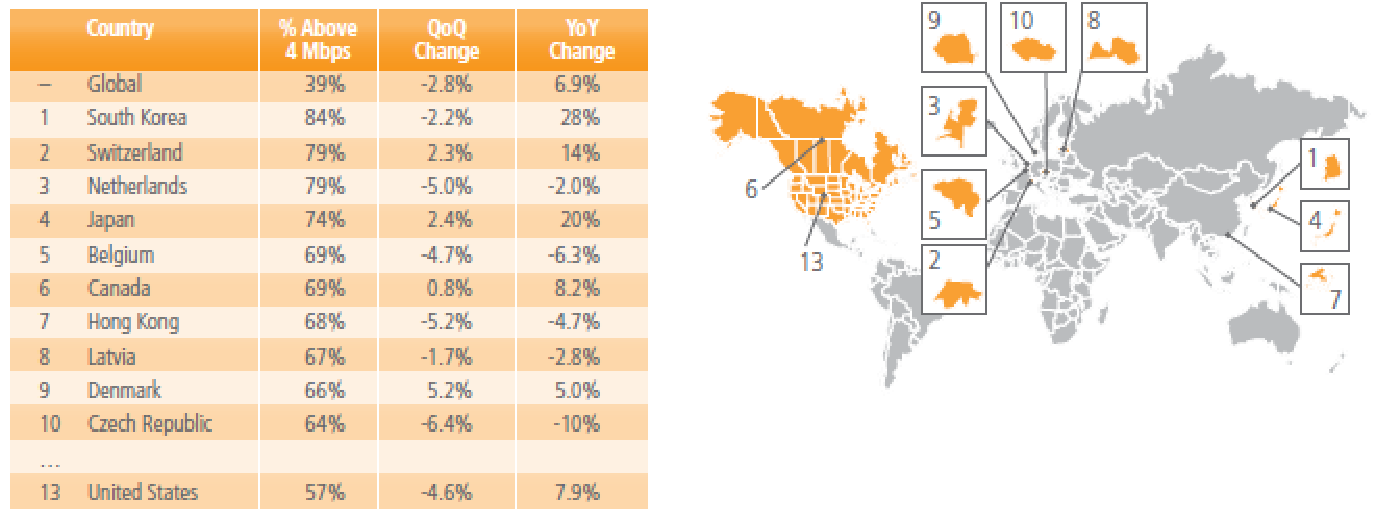
\includegraphics[width=1\textwidth]{./figures/internetstats.pdf}
      \caption[Broadband over 4Mbps connectivity statistics]{Broadband connectivity statistics about the speeds over 4Mbps around the globe.}
\end{figure}

